\documentclass[a4paper,11pt]{article}

\usepackage[T1]{fontenc}
\usepackage{lmodern}
\usepackage[margin=2.5cm]{geometry}
\usepackage{graphicx}
\usepackage{float}
\usepackage{xcolor}
\usepackage{booktabs}
\usepackage{tabularx}
\usepackage{enumitem}
\usepackage{lastpage}
\usepackage{fancyhdr}
\usepackage{tikz}
\usetikzlibrary{positioning,arrows.meta}
\usepackage[colorlinks=true,urlcolor=mhgold,linkcolor=black]{hyperref}

\definecolor{mhgold}{HTML}{B8860B}
\definecolor{mhdark}{HTML}{1B2433}
\definecolor{mhlight}{HTML}{F6F1E4}
\definecolor{mhblue}{HTML}{3B5BDB}
\definecolor{mhgrey}{HTML}{5A6670}

\pagestyle{fancy}
\fancyhf{}
\fancyhead[L]{\small\color{mhgrey} MH Dashboard: Technical Overview}
\fancyhead[R]{\small\color{mhgrey} G\"orkem \"Ozbek}
\fancyfoot[C]{\small\color{mhgrey} \thepage\ / \pageref{LastPage}}
\renewcommand{\headrulewidth}{0.3pt}

\setlength{\parindent}{0pt}
\setlength{\parskip}{0.6em}
\setlist{itemsep=0.15em, topsep=0.3em}
\newcommand{\code}[1]{\texttt{#1}}

\begin{document}

%================ TITLE ================
\thispagestyle{empty}
\begin{center}
\vspace*{2.5cm}
{\fontsize{34}{40}\selectfont\bfseries\color{mhdark} MH Dashboard}\\[0.7em]
{\Large Stock, order and sales intelligence}\\[0.3em]
{\Large for a luxury drinks distributor}\\[2em]
{\large Technical overview of an internal production tool}\\[0.4em]
{\color{mhgrey} Built for Mo\"et Hennessy T\"urkiye}\\[2.5em]
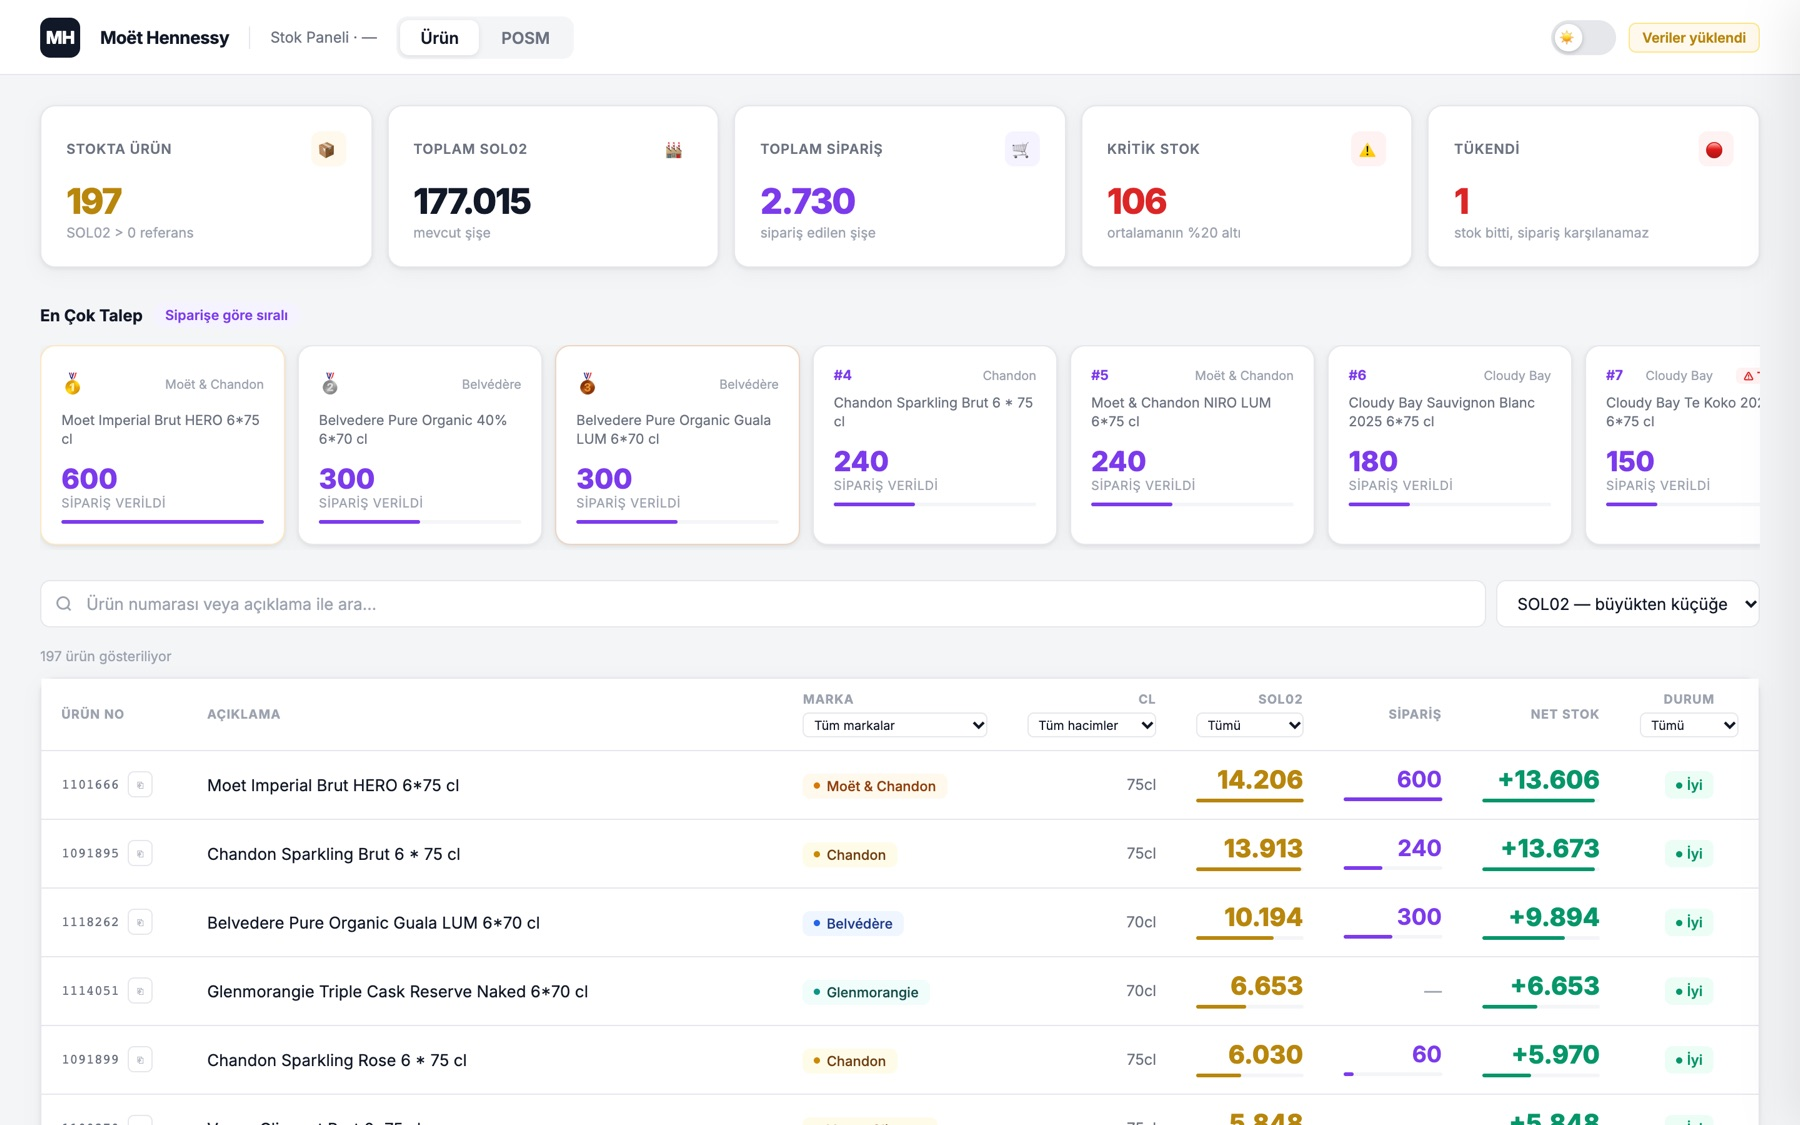
\includegraphics[width=\linewidth]{../screenshots/01-products.jpg}\\[3em]
{\large\bfseries G\"orkem \"Ozbek}\\[0.3em]
{\color{mhgrey} Galatasaray University \textperiodcentered{} 2026}
\end{center}
\newpage

\tableofcontents
\newpage

%================ 1 ================
\section{Overview}

MH Dashboard is a web application that gives the stock and sales team of a luxury drinks distributor one live view of their products, point-of-sale materials (POSM) and orders. It collects data from the company's systems (SAP, shared Excel files and order records), cleans and classifies it, and turns it into indicators, alerts, rankings, forecasts and AI-generated analyses.

I designed and built the whole tool, from data ingestion to the user interface, and it is used in production.

\begin{center}
\fbox{\parbox{0.9\linewidth}{\small This is an internal company tool: its source code and live data are private. The screenshots in this document come from the production dashboard.}}
\end{center}

%================ 2 ================
\section{The Problem}

The distributor sells many brands (Mo\"et \& Chandon, Dom P\'erignon, Veuve Clicquot, Krug, Ruinart, Hennessy, Glenmorangie, Ardbeg, Belv\'ed\`ere, Cloudy Bay and others), each with several products and bottle sizes, plus a large catalogue of POSM: glasses, ice buckets, trays, displays and bar tools.

Before the dashboard, the data was spread across:
\begin{itemize}
  \item the \textbf{SAP} ERP for official stock and movements;
  \item \textbf{Excel exports} shared on SharePoint, with free-text descriptions;
  \item separate \textbf{order} records.
\end{itemize}
Simple questions such as \emph{``Which products will run out soon?''}, \emph{``What is ordered the most?''} or \emph{``How much should we order next month?''} required opening several files and combining them by hand.

%================ 3 ================
\section{Features}

\begin{figure}[H]
\centering
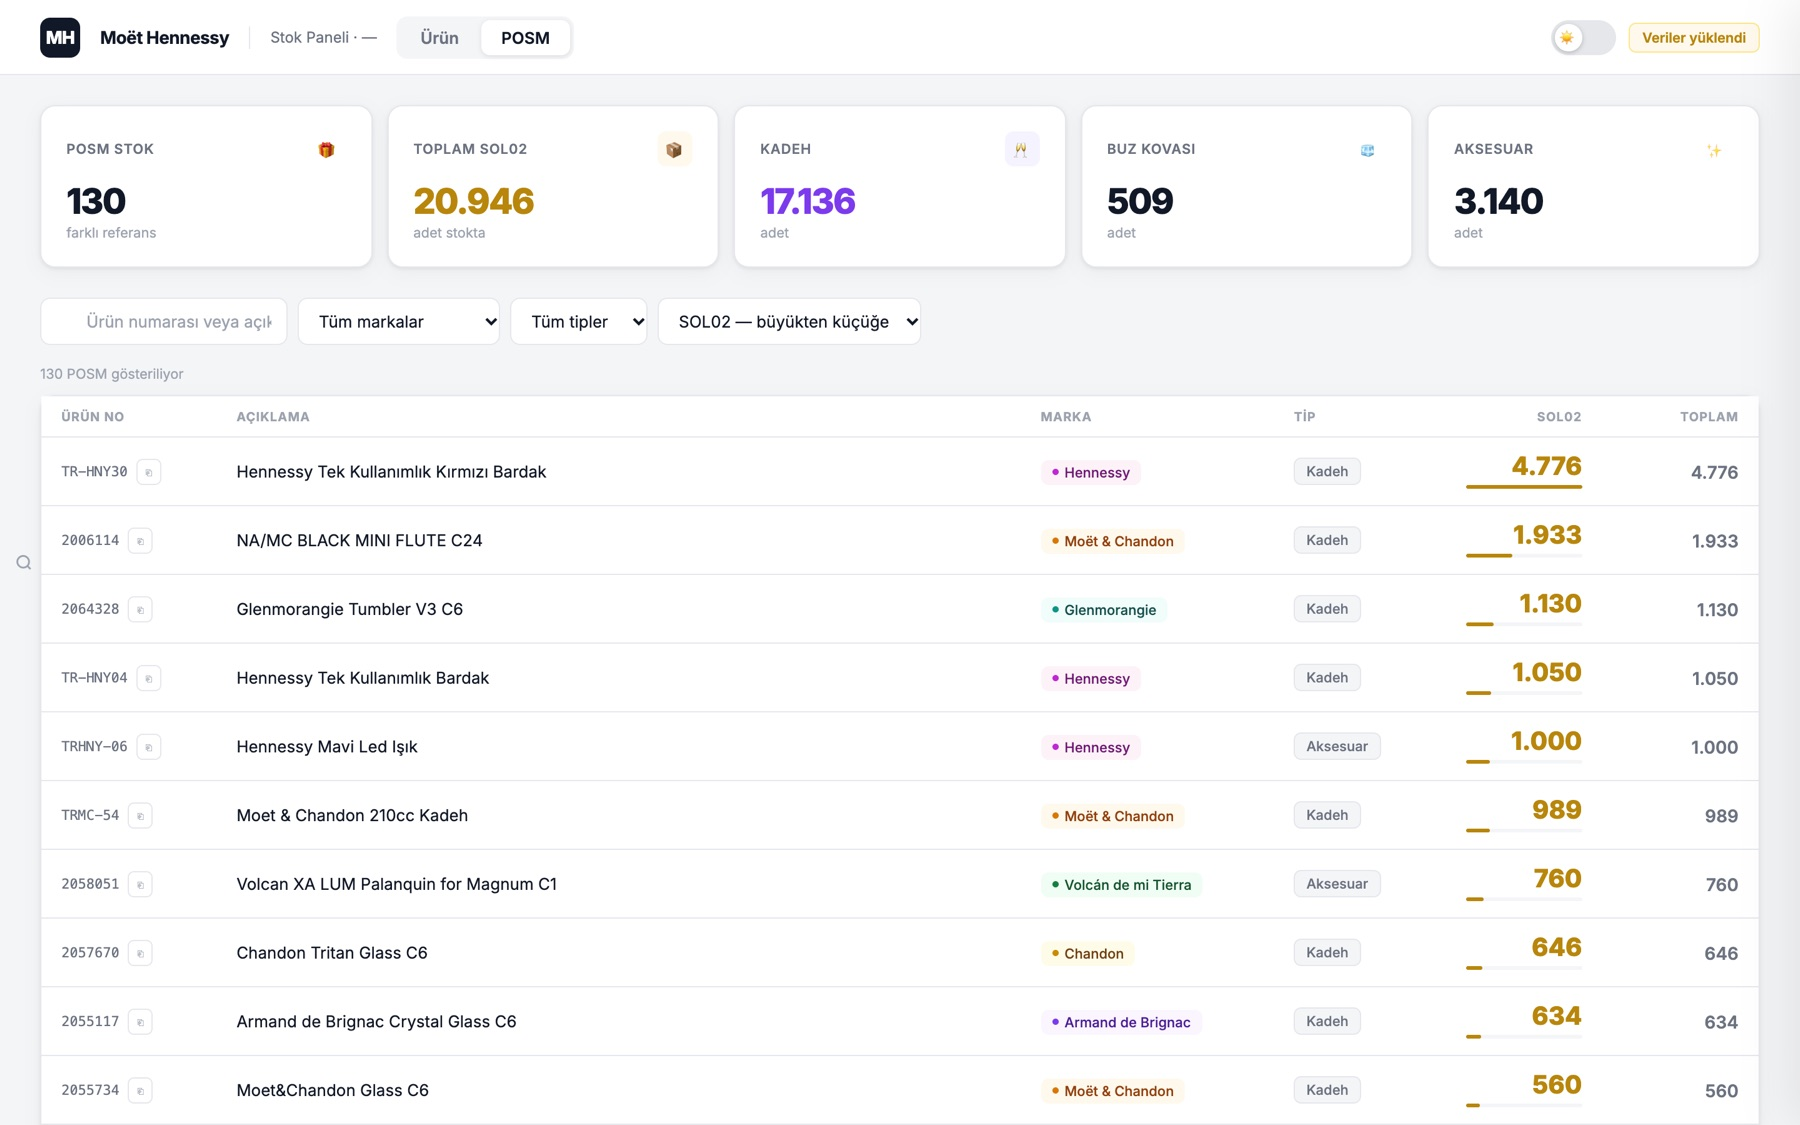
\includegraphics[width=\linewidth]{../screenshots/02-posm.jpg}
\caption{POSM view: stock of point-of-sale materials by type and brand.}
\end{figure}

\subsection{Data integration}
\begin{itemize}
  \item \textbf{SAP integration}: stock and movement data from the company ERP.
  \item \textbf{Automatic Excel sync}: the shared stock file on SharePoint is fetched by the server, parsed, and cached for 15 minutes, so the dashboard is always close to real time without overloading the source.
  \item \textbf{Excel import}: a full stock export (\code{.xlsx}) can be uploaded and is merged on the server.
  \item \textbf{Classification}: each line is classified automatically (Section~\ref{sec:classif}).
\end{itemize}

\subsection{Stock and orders}
\begin{itemize}
  \item \textbf{Key indicators}: number of products in stock, total bottles, total ordered, critical stock, out of stock.
  \item \textbf{Critical stock}: products below 20\% of the average stock level, and products whose stock can no longer cover their orders.
  \item \textbf{Automatic order tracking}: orders are followed until delivery, and their effect on stock is computed for each product (\emph{net stock} = stock $-$ open orders).
  \item \textbf{Search and filters} by reference, description, brand, bottle size, stock level and status.
  \item \textbf{POSM view} grouped by material type and brand.
\end{itemize}

\subsection{Analytics and AI}
\begin{itemize}
  \item \textbf{Best and worst sellers}: ranking of the most and least ordered products, by brand and by period.
  \item \textbf{Sales forecasting}: expected demand per product, to plan orders before stock runs out.
  \item \textbf{AI analyst}: questions about the data in plain language, answered with summaries and recommendations.
\end{itemize}

\subsection{Team features}
\begin{itemize}
  \item \textbf{Notes and photos} attached to a product and shared with the team.
  \item \textbf{Light and dark mode}.
  \item \textbf{Password-protected access}, with the stock data stored encrypted (AES-256).
  \item \textbf{Usage analytics} to see which parts of the tool the team uses.
\end{itemize}

\begin{figure}[H]
\centering
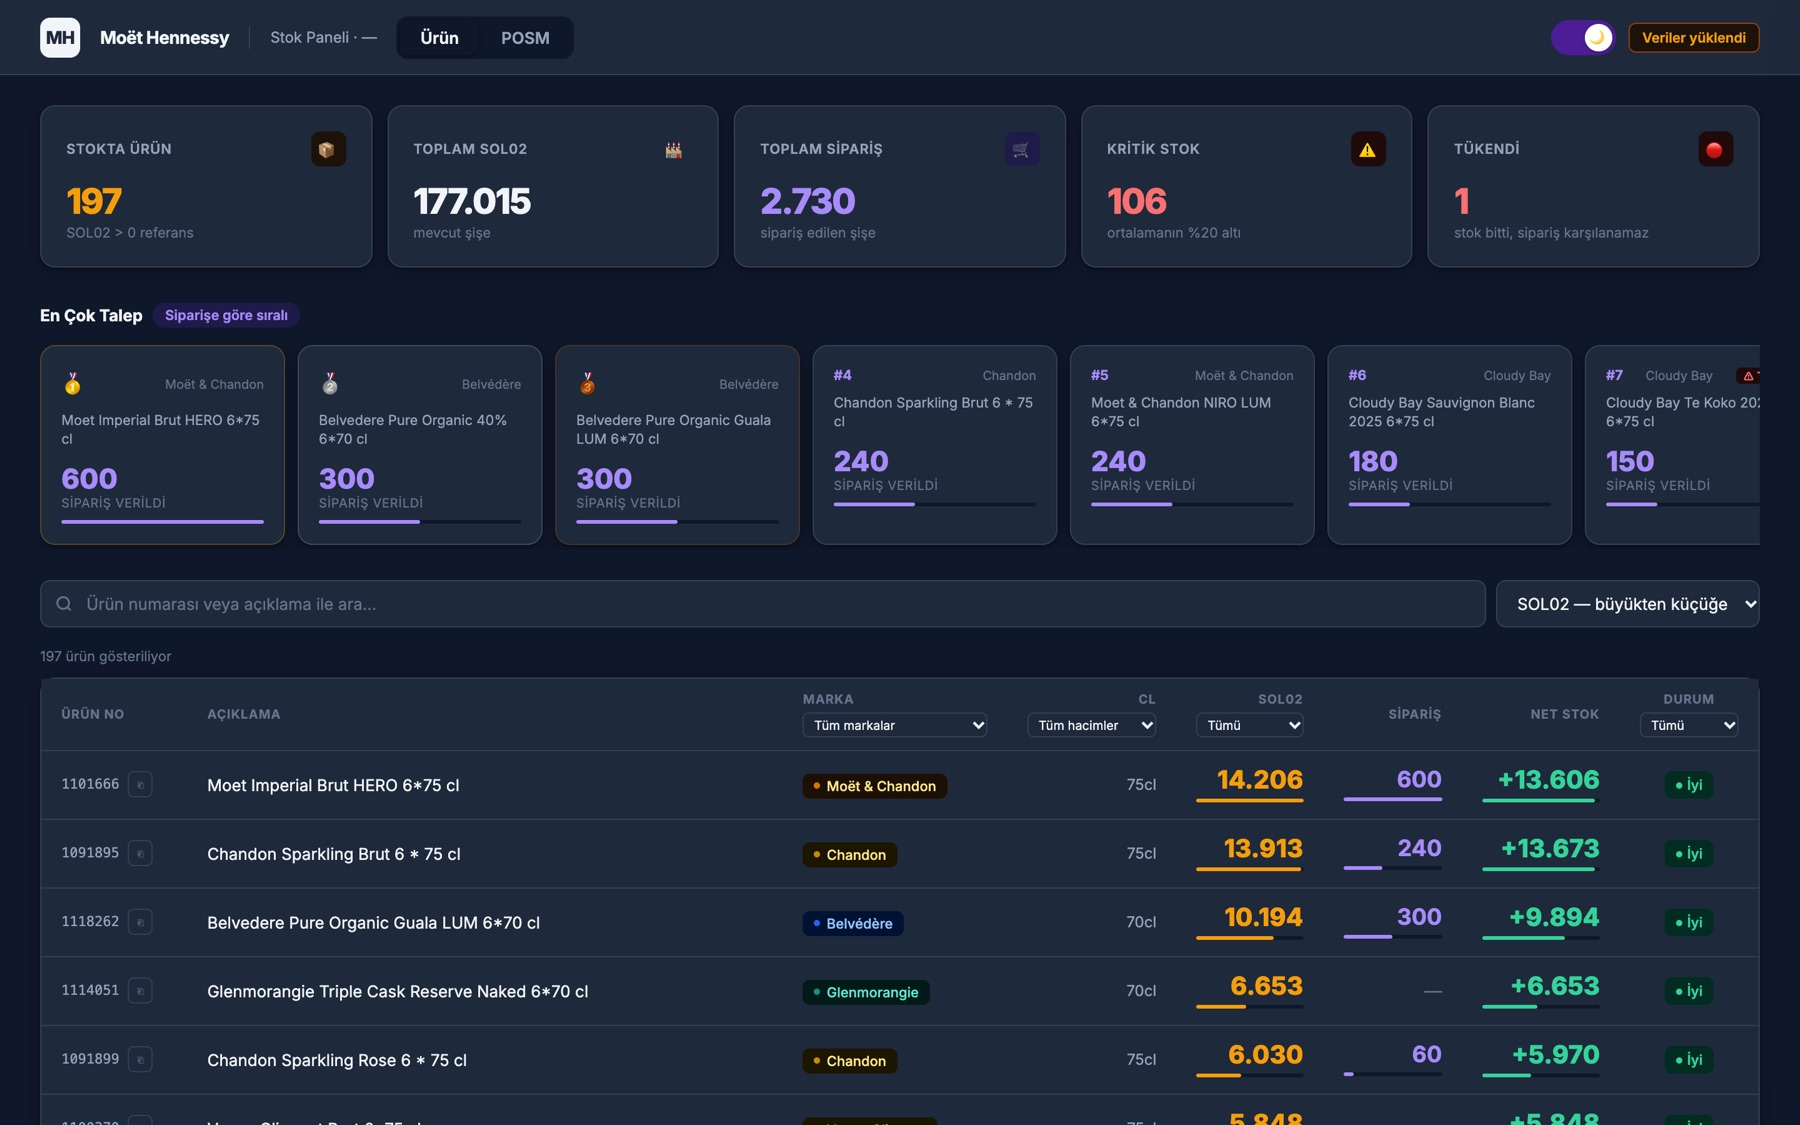
\includegraphics[width=0.95\linewidth]{../screenshots/03-dark-mode.jpg}
\caption{Dark mode of the products view.}
\end{figure}

%================ 4 ================
\section{Architecture}

\begin{figure}[H]
\centering
\resizebox{\linewidth}{!}{%
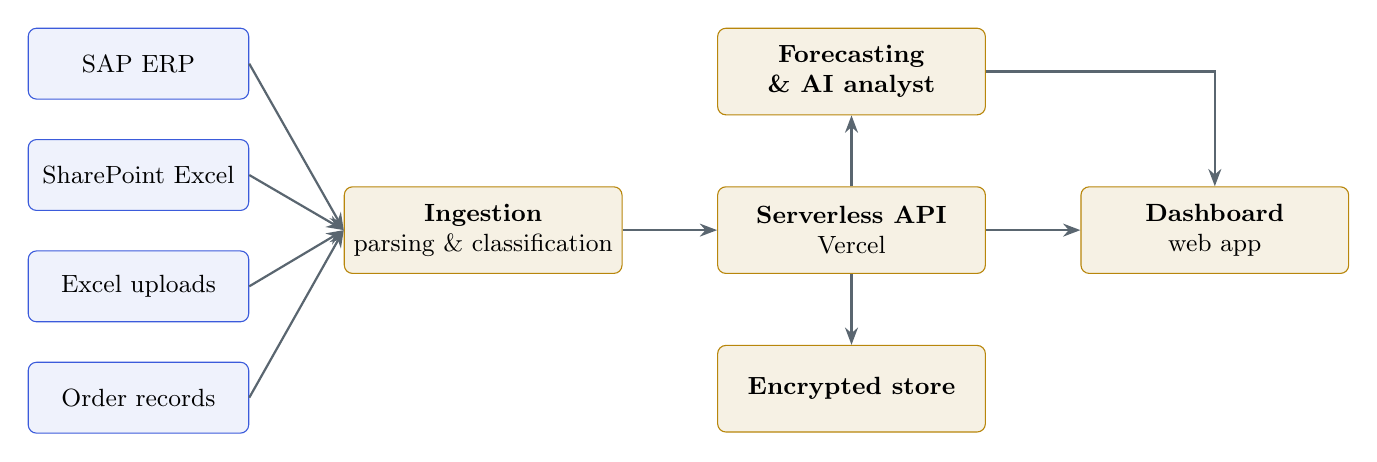
\begin{tikzpicture}[
  node distance=0.5cm and 1.2cm,
  src/.style={draw=mhblue, fill=mhblue!8, rounded corners=3pt, align=center, minimum width=2.8cm, minimum height=0.9cm, font=\small},
  box/.style={draw=mhgold, fill=mhlight, rounded corners=3pt, align=center, minimum width=3.4cm, minimum height=1.1cm, font=\small},
  arr/.style={-{Stealth[length=2.2mm]}, thick, color=mhgrey}
]
\node[src] (sap) {SAP ERP};
\node[src, below=of sap] (sp) {SharePoint Excel};
\node[src, below=of sp] (xl) {Excel uploads};
\node[src, below=of xl] (ord) {Order records};
\node[box, right=of sp, yshift=-0.7cm] (ing) {\textbf{Ingestion}\\parsing \& classification};
\node[box, right=of ing] (api) {\textbf{Serverless API}\\Vercel};
\node[box, above=0.9cm of api] (an) {\textbf{Forecasting}\\\textbf{\& AI analyst}};
\node[box, below=0.9cm of api] (db) {\textbf{Encrypted store}};
\node[box, right=of api] (ui) {\textbf{Dashboard}\\web app};
\foreach \s in {sap,sp,xl,ord} \draw[arr] (\s.east) -- (ing.west);
\draw[arr] (ing) -- (api);
\draw[arr] (api) -- (db);
\draw[arr] (api) -- (an);
\draw[arr] (api) -- (ui);
\draw[arr] (an) -| (ui);
\end{tikzpicture}}
\caption{Data flow from the company sources to the dashboard.}
\end{figure}

\textbf{Frontend.} A single-page application written in plain HTML, CSS and JavaScript, without a framework, so it loads fast and is easy to deploy. It handles login, the product and POSM views, filters, sorting, notes and the theme.

\textbf{Backend.} Node.js serverless functions on Vercel: data retrieval, updates, Excel import, the SharePoint proxy, notes, analytics, forecasting and the AI analyst. Secrets are stored as environment variables on the server.

\textbf{Storage.} The stock data is stored as an encrypted JSON document and every change is versioned, which gives a full history of updates. When two people save at the same time, the server detects the conflict and retries the update on the latest version instead of overwriting it.

%================ 5 ================
\section{Data Cleaning and Classification}\label{sec:classif}

The source files describe products in free text written by different people, for example \emph{``NA/MC BLACK MINI FLUTE C24''} or \emph{``Belvedere Pure Organic 40\% 6*70 cl''}. The ingestion step turns each line into a structured record:

\begin{itemize}
  \item \textbf{Brand}: detected in three steps, from the most to the least reliable: internal prefixes (for example \code{NA/MC} or \code{SC/DP}), then short brand codes at the start of the description, then brand names and well-known product names anywhere in the text (for example \emph{La Grande Dame} for Veuve Clicquot). More than 25 brands are recognised.
  \item \textbf{Bottle size}: extracted from patterns such as \code{6*75 cl} or \code{70cl}.
  \item \textbf{Product or POSM}: decided from the reference prefixes and the description.
  \item \textbf{POSM type}: glass, ice bucket, tray, display, pitcher, bar mat, bar tool, book or accessory, from keywords in several languages (English, French, Turkish).
\end{itemize}
These rules were built from the real product catalogue and refined each time a new type of line appeared.

%================ 6 ================
\section{Indicators and Alerts}

\begin{tabularx}{\linewidth}{@{}lX@{}}
\toprule
\textbf{Indicator} & \textbf{Definition} \\
\midrule
Products in stock & Number of references with a positive stock \\
Total stock & Sum of bottles in stock \\
Total ordered & Sum of bottles in open orders \\
Net stock & Stock $-$ open orders, per product \\
Critical stock & Products below 20\% of the average stock level \\
Out of stock & Products whose stock cannot cover their orders \\
Top demand & Products ranked by ordered quantity \\
\bottomrule
\end{tabularx}

%================ 7 ================
\section{Impact}

\begin{itemize}
  \item The team sees stock, orders and alerts in \textbf{one place, in seconds}, instead of combining several Excel files.
  \item Shortages are visible \textbf{before} they happen, thanks to the critical-stock and net-stock indicators.
  \item Forecasts and AI summaries help to \textbf{plan orders} and to report to managers.
\end{itemize}

%================ 8 ================
\section{What I Learned}

\begin{itemize}
  \item Integrating data from an ERP, spreadsheets and manual files into one clean model.
  \item Writing robust cleaning and classification rules for real, messy business data.
  \item Building a tool for real users inside a company, and improving it from their feedback.
  \item Serverless design: caching, safe concurrent updates and encrypted storage.
  \item Turning raw data into decisions with indicators, alerts, forecasting and AI.
\end{itemize}

\section{Next Steps}
\begin{itemize}
  \item Generalise the platform to other companies and data sources (\emph{DataLens}).
  \item Move from a document store to a relational database for larger datasets.
  \item Role-based access for different teams.
\end{itemize}

\end{document}
